\documentclass{standalone}
%
\usepackage{tikz}
\usepackage{xcolor}
%
\definecolor{craterm}{HTML}{616060}
%
\title{Trisecare un foglio di carta}
\begin{document}
	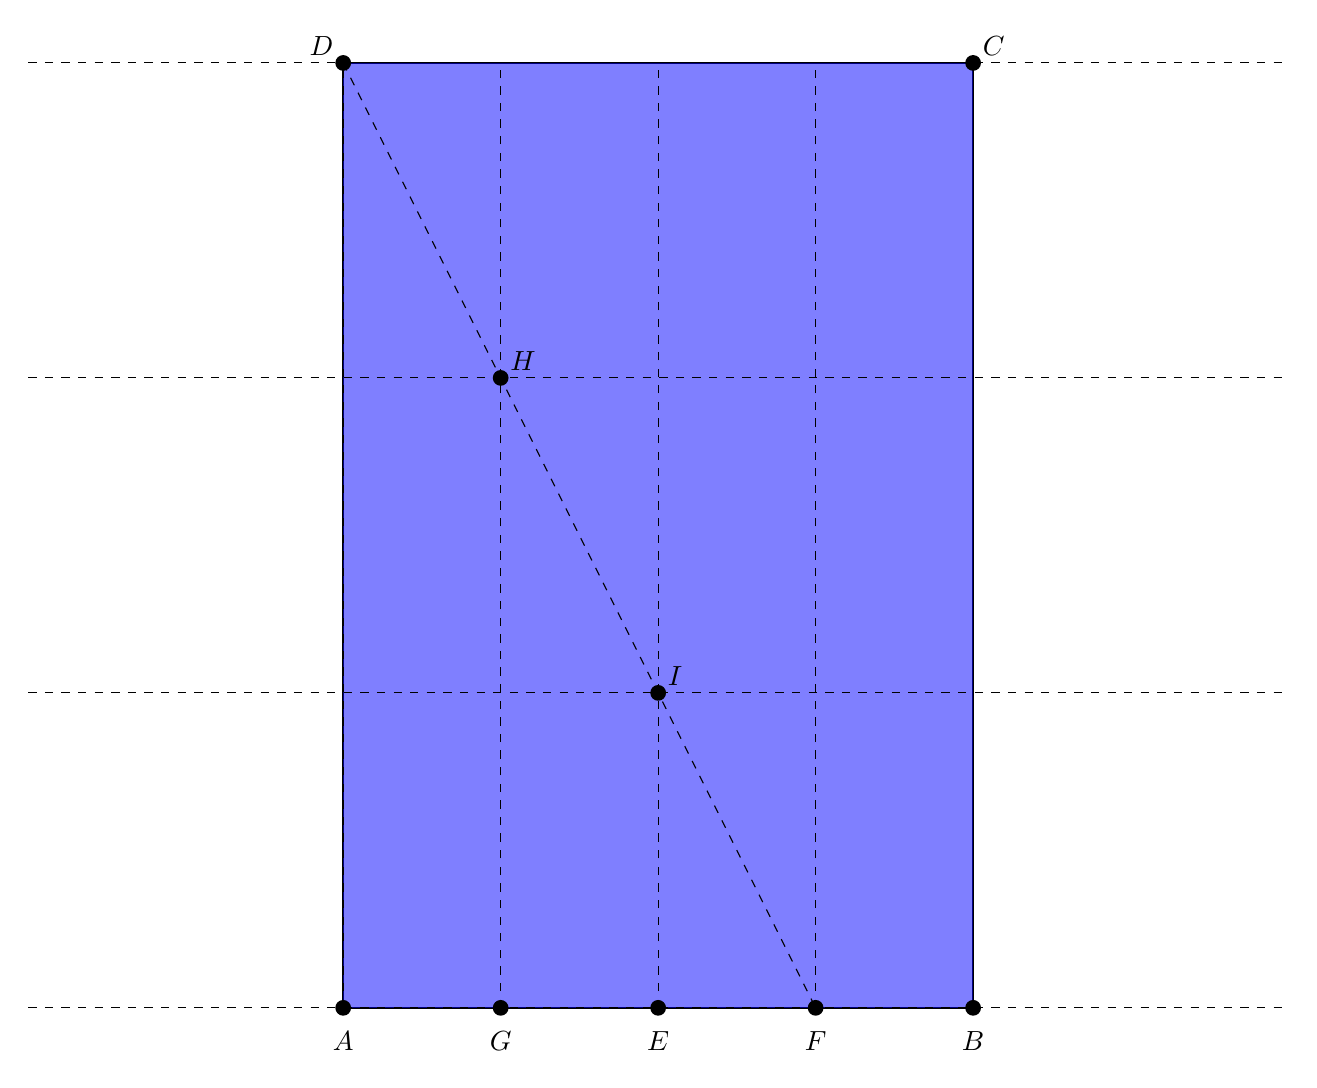
\begin{tikzpicture}
		\begin{scope}[scale=2]
			\draw [thick] (2,0) rectangle (6,6);
			\fill [blue, opacity=0.5] (2,0) rectangle (6,6);
			\foreach \y in {0,2,4,6}
				\draw [-,dashed] (0,\y) -- (8,\y);
			\foreach \x in {2,3,...,6}{
				\draw [-,dashed] (\x,0) -- (\x,6);
				\fill [black] (\x,0) circle (0.05cm);
			}
			\fill [black] (4,2) circle (0.05cm);
			\fill [black] (3,4) circle (0.05cm);
			\fill [black] (2,6) circle (0.05cm);
			\fill [black] (6,6) circle (0.05cm);
			\draw [-,dashed] (2,6) -- (5,0);
			%
			\node [below=5] at (2,0) {$A$};
			\node [below=5] at (6,0) {$B$};
			\node [above=6,right] at (6,6) {$C$};
			\node [above=6,left] at (2,6) {$D$};
			\node [below=5] at (4,0) {$E$};
			\node [below=5] at (5,0) {$F$};
			\node [below=5] at (3,0) {$G$};
			\node [above=6,right] at (3,4) {$H$};
			\node [above=6,right] at (4,2) {$I$};
		\end{scope}
	\end{tikzpicture}
\end{document}